% ju 17-Feb-24 Mars-Rover.tex
\documentclass{vorlage-design-main}
\usepackage[utf8]{inputenc}
\usepackage{longtable}
\usepackage{blindtext,alltt}
%% Ganze Überschrift
\title{Thema}

%% Kürzerer Titel zur Verwendung im Seitenkopf
\runningtitle{Kurztitel}
\author{Jan Unger}
% \author{2.}
\date{\today}

%% Die .bib-Datei mit vollständigen Referenzen zur Verwendung mit biblatex. articleclass lädt das Paket biblatex-chicago mit Anpassungen
\addbibresource{literatur.bib}

\begin{document}

\maketitle

\begin{abstract}

\end{abstract}

\begin{figure}
\centering
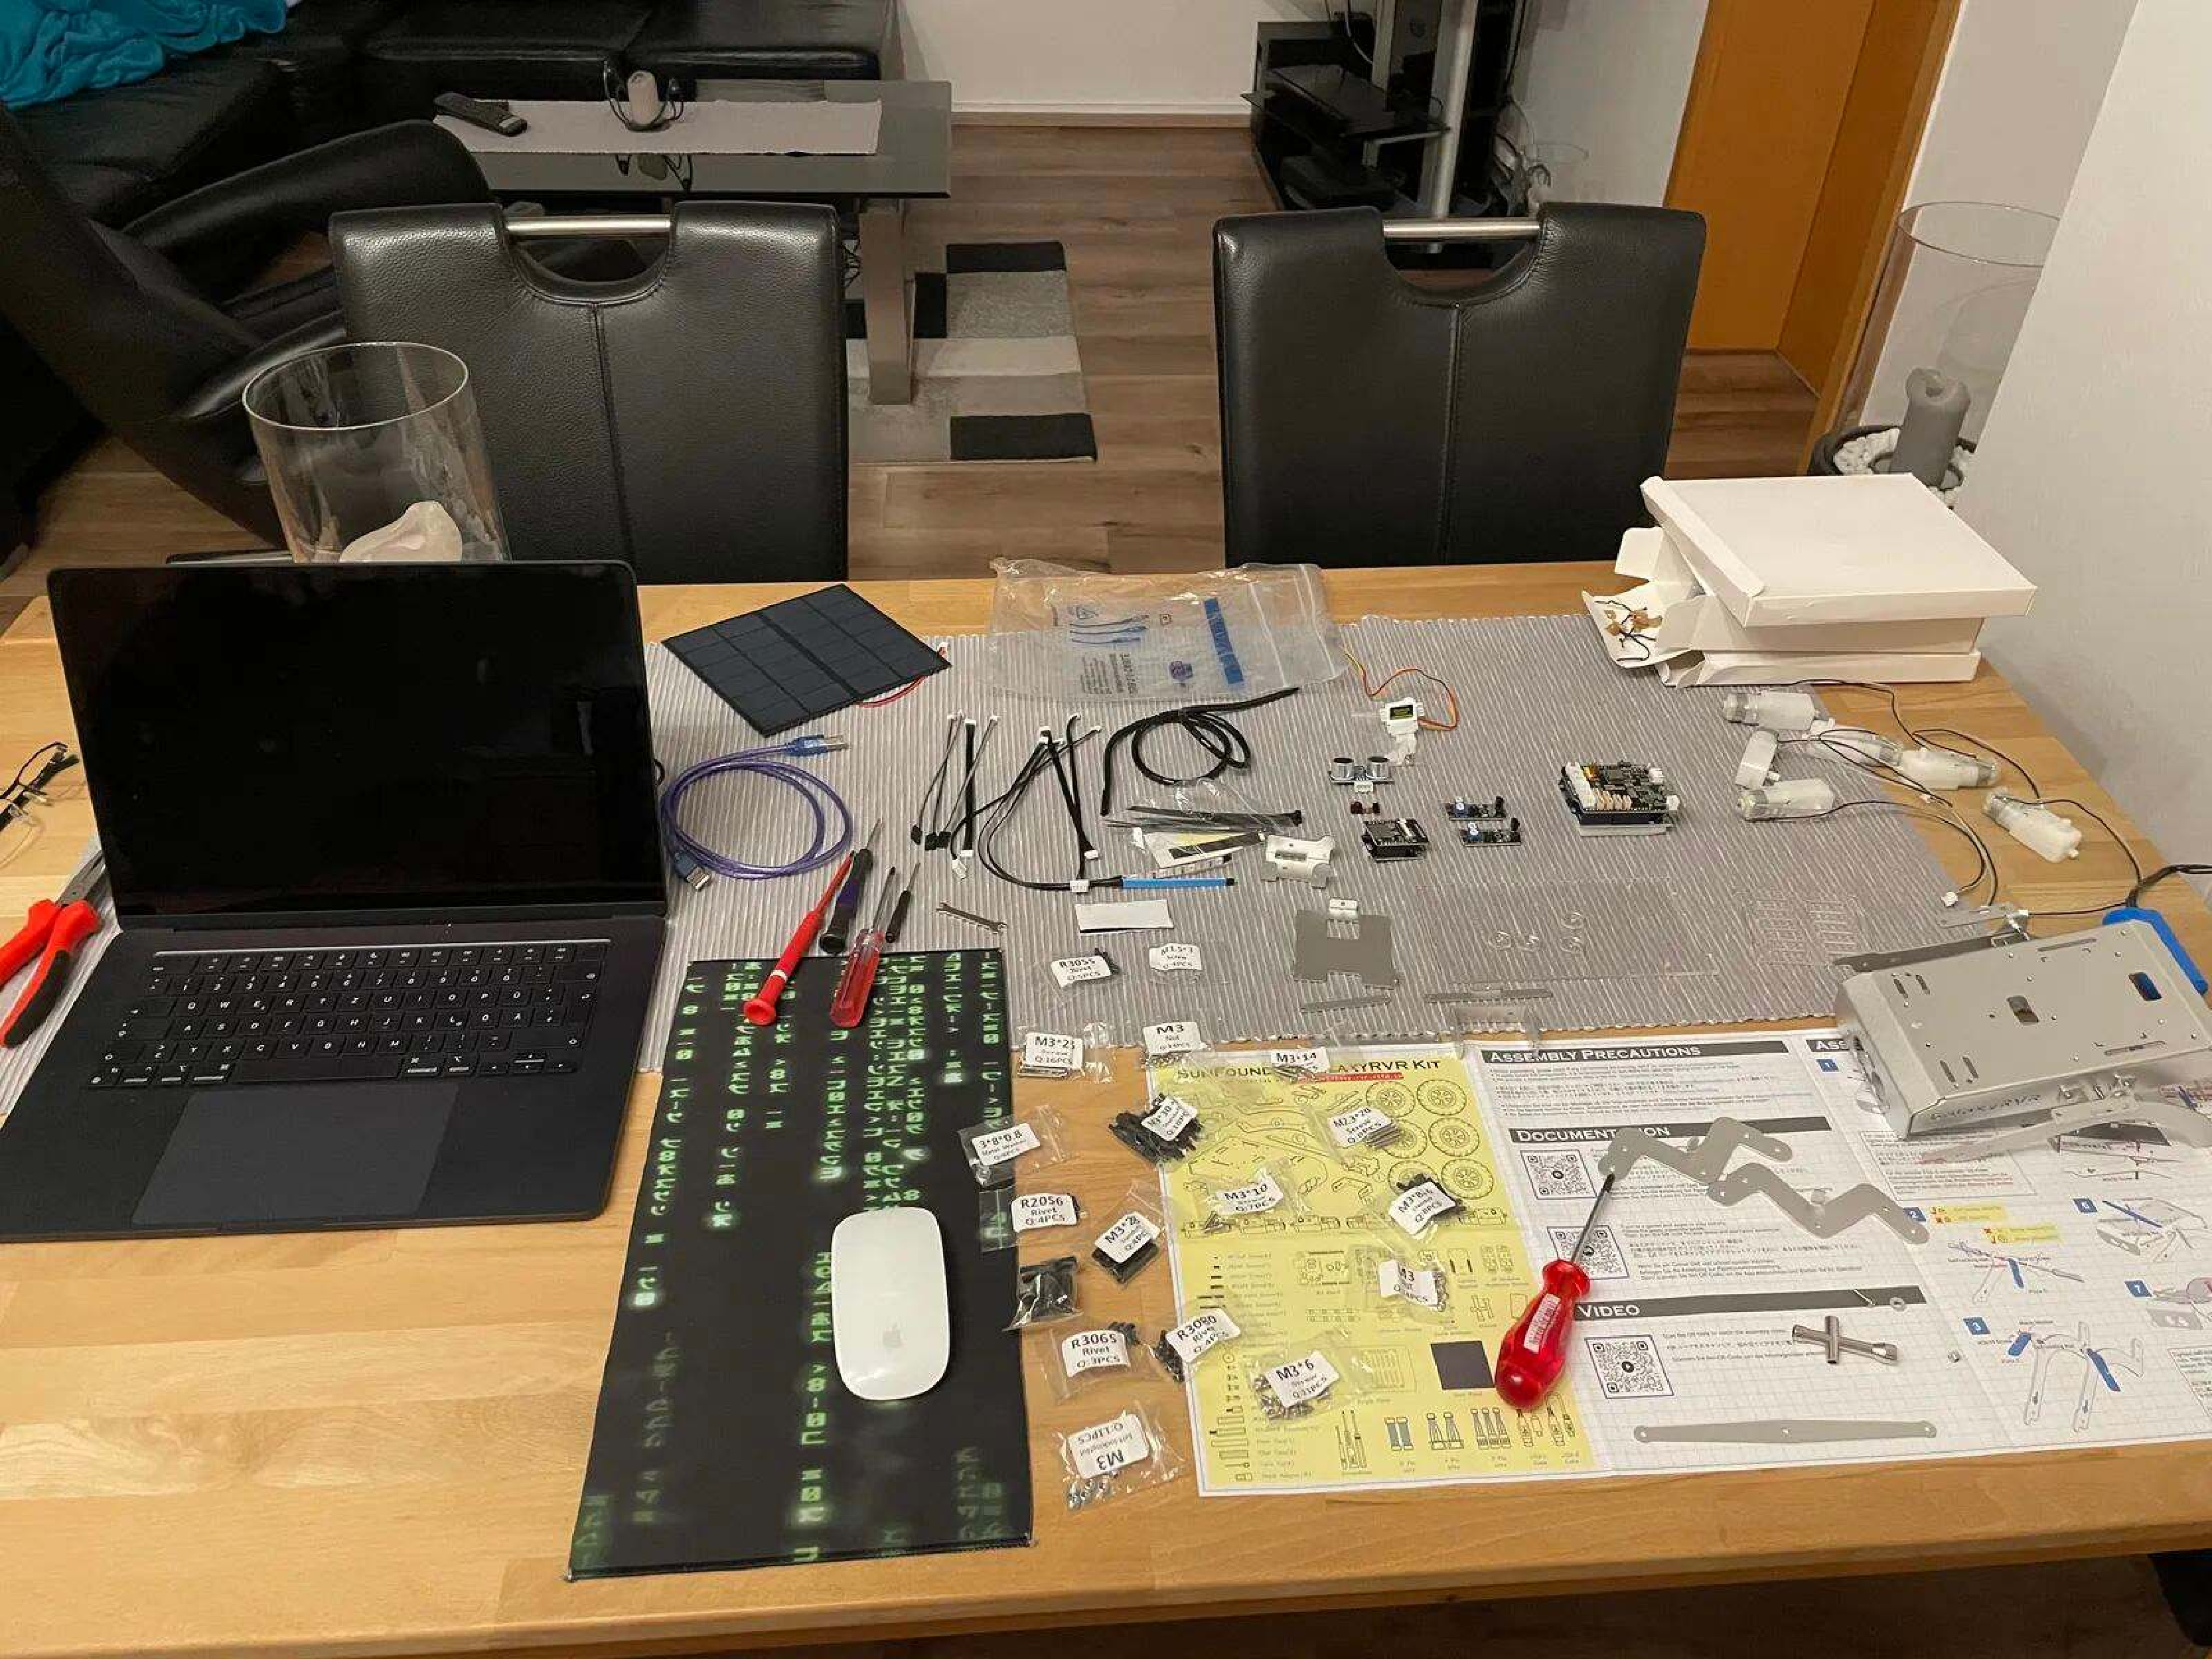
\includegraphics[width=0.8\textwidth]{images/rover-bau.pdf}
\floatnotes{}
%\label{fig:}
\caption{Mars-Rover Montage}
\end{figure}

\begin{figure}
\centering
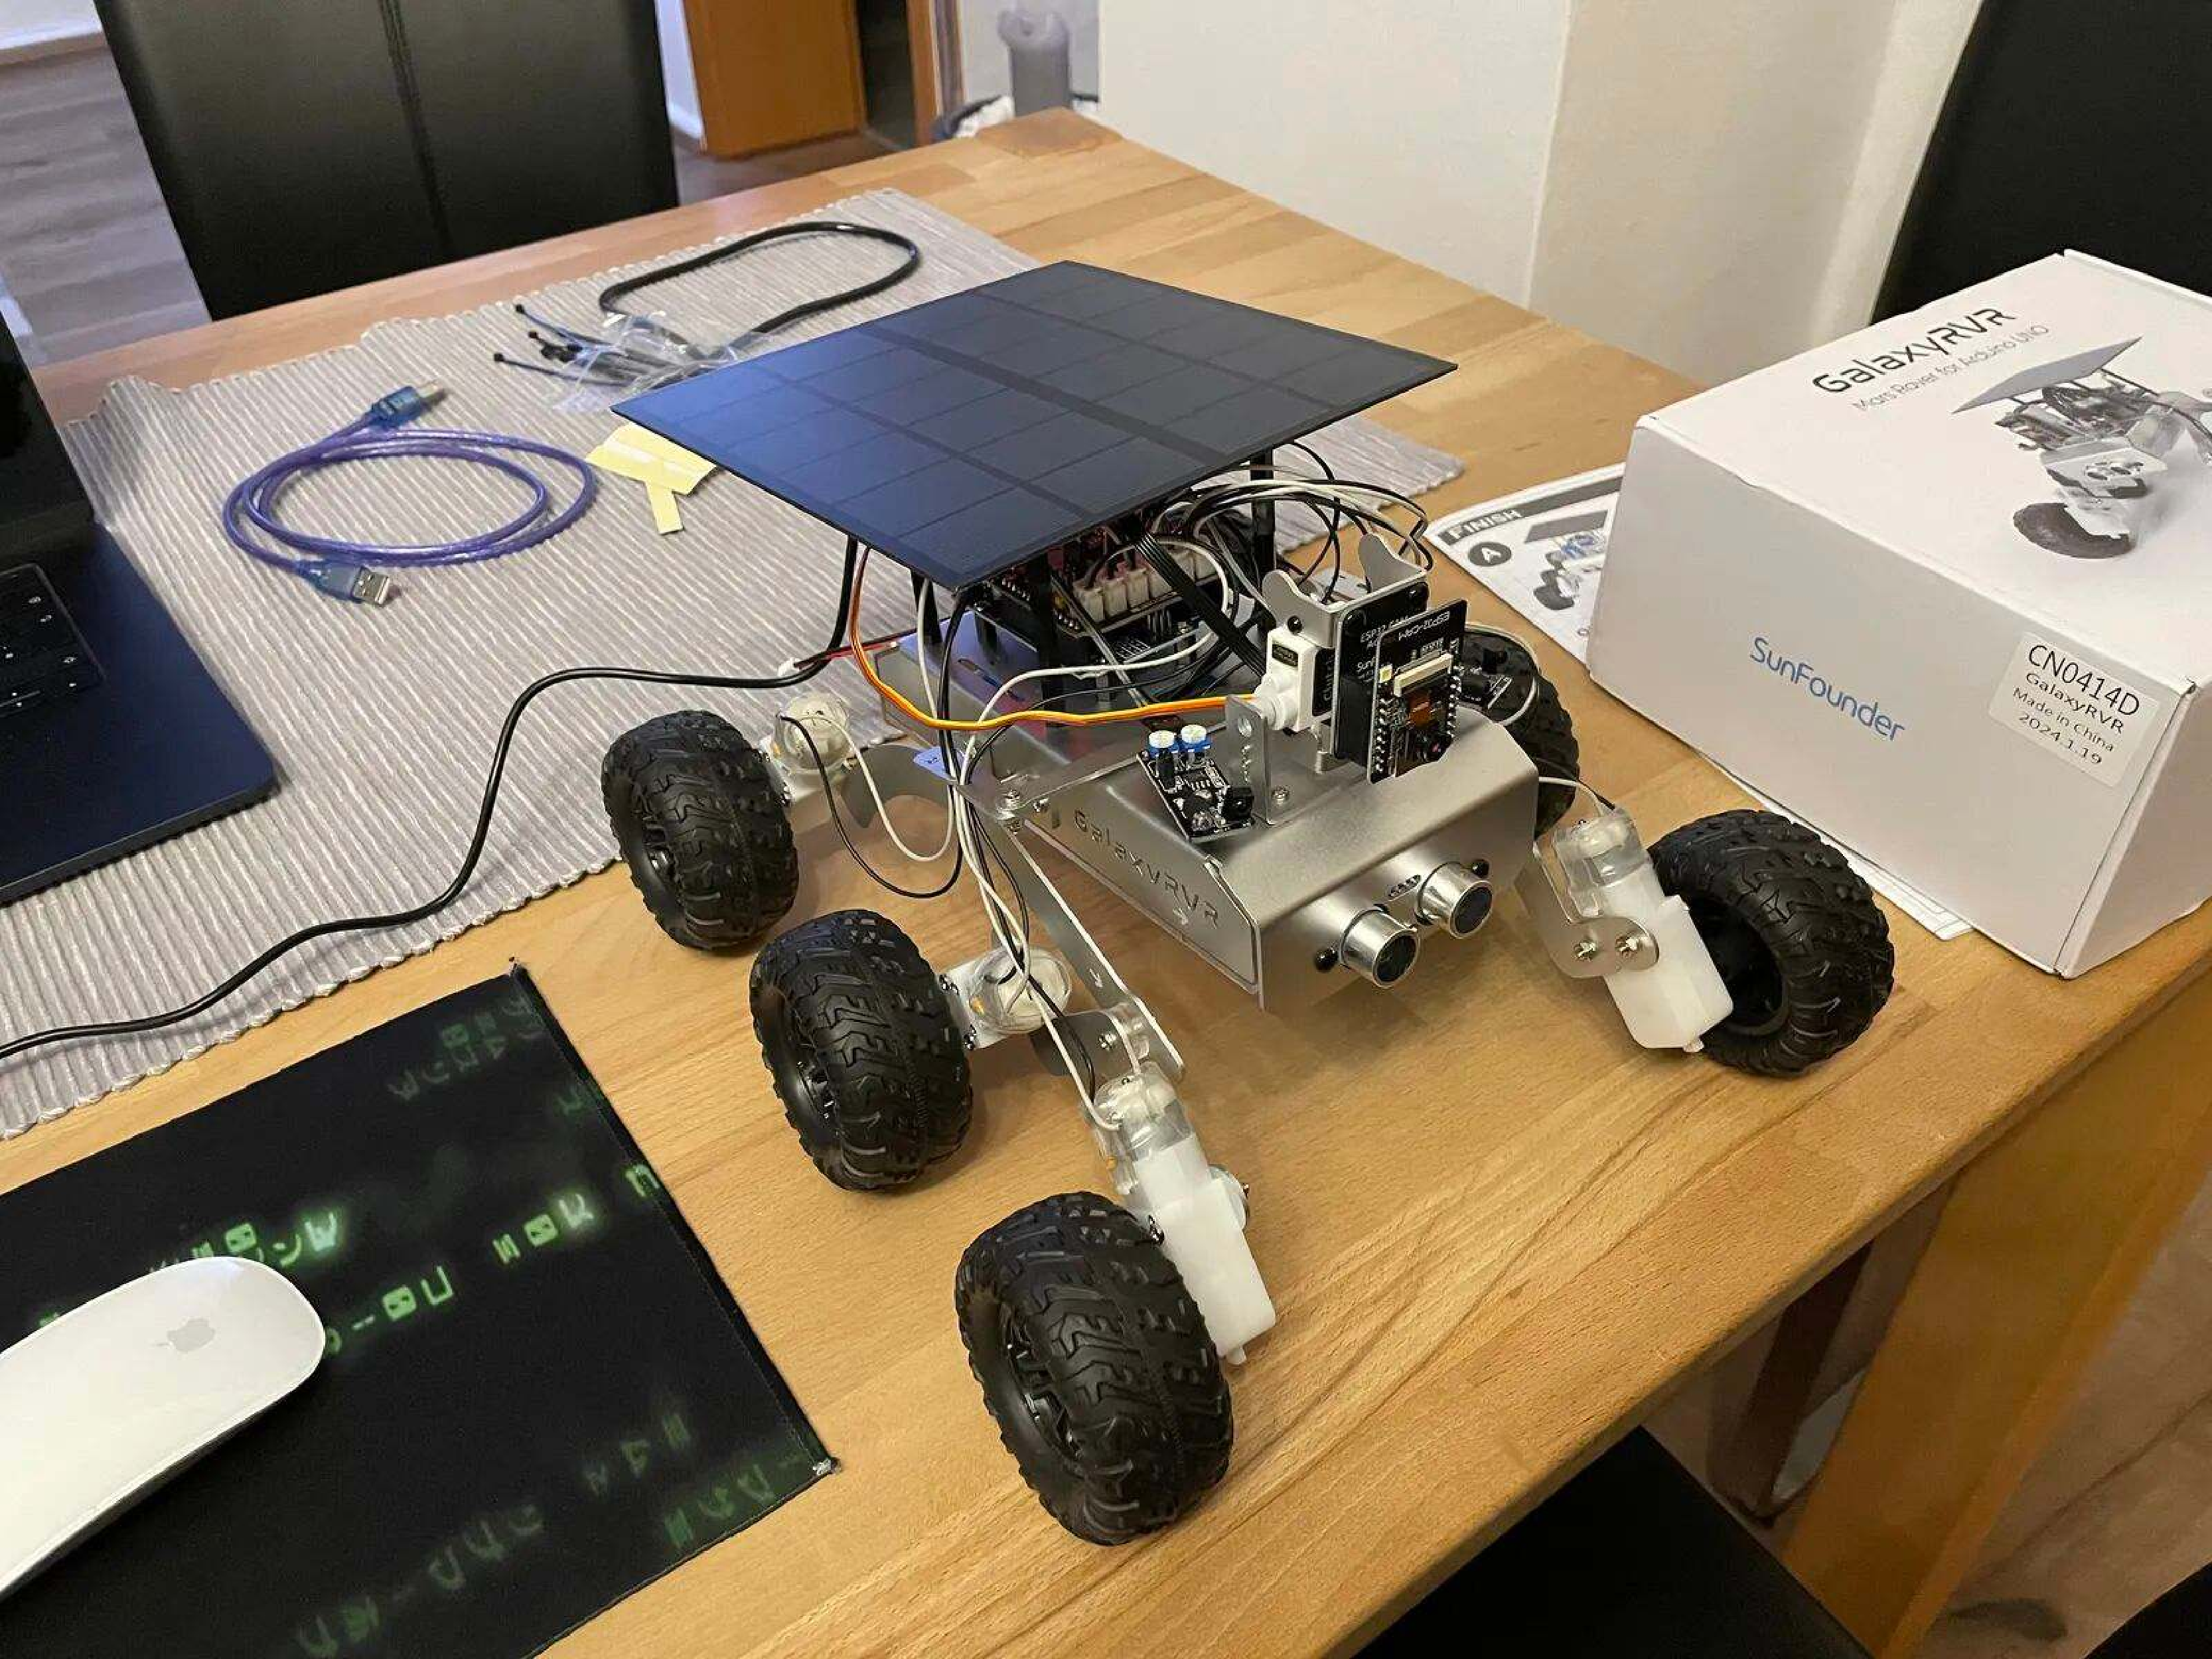
\includegraphics[width=0.8\textwidth]{images/rover-bau2.pdf}
\floatnotes{}
%\label{fig:}
\caption{Mars-Rover Montage 2}
\end{figure}

\hypertarget{enthuxfcllung-des-mars-rovers}{%
\subsection{Enthüllung des
Mars-Rovers}\label{enthuellung-des-mars-rovers}}

\hypertarget{unterschiede-in-den-designs}{%
\subsubsection{Unterschiede in den
Designs}\label{unterschiede-in-den-designs}}

\begin{itemize}

\item
  \textbf{Sojourner (1997)}: Als erster Rover auf dem Mars klein und
  relativ einfach gestaltet, mit dem Hauptziel, die Machbarkeit der
  Rover-Technologie auf dem Mars zu demonstrieren.
\item
  \textbf{Spirit und Opportunity (2004)}: Beide hatten ein
  ausgeklügelteres Design als Sojourner, waren größer, hatten eine
  längere Missionsdauer und waren mit fortschrittlicheren
  wissenschaftlichen Instrumenten ausgestattet, um Geologie und
  Atmosphäre zu erforschen.
\item
  \textbf{Curiosity (2012)}: Noch größer und komplexer, mit einem Labor
  an Bord, um chemische Analysen durchzuführen und nach Bedingungen für
  mikrobielles Leben zu suchen.
\item
  \textbf{Perseverance (2021)}: Baut auf Curiositys Design auf, mit
  zusätzlichen Instrumenten für astrobiologische Forschung,
  einschließlich der Suche nach fossilen Mikroben, und dem
  experimentellen Mars-Hubschrauber Ingenuity.
\end{itemize}

\hypertarget{gemeinsamkeiten}{%
\subsubsection{Gemeinsamkeiten}\label{gemeinsamkeiten}}

\begin{itemize}

\item
  Alle Rover sind mit Kameras und wissenschaftlichen Instrumenten
  ausgestattet, um den Mars zu studieren.
\item
  Solarenergie (bis Curiosity, der mit einem Radioisotopengenerator
  betrieben wird) und Kommunikationsfähigkeit mit der Erde.
\item
  Mobilität auf der Oberfläche zur Durchführung geologischer
  Untersuchungen und Atmosphärenmessungen.
\end{itemize}

\hypertarget{einfluss-der-missionsziele-auf-das-design}{%
\subsubsection{Einfluss der Missionsziele auf das
Design}\label{einfluss-der-missionsziele-auf-das-design}}

\begin{itemize}

\item
  Mit jedem Rover wuchsen die Missionsziele, was zu komplexeren Designs
  führte. Während Sojourner hauptsächlich die Technologie testete,
  suchten spätere Rover nach Wasserzeichen, aktuellen und vergangenen
  Lebensbedingungen und bereiteten die Mars-Erkundung durch Menschen
  vor.
\item
  Die Instrumentenauswahl reflektiert die spezifischen
  wissenschaftlichen Ziele jeder Mission.
\end{itemize}

\hypertarget{technologische-fortschritte}{%
\subsubsection{Technologische
Fortschritte}\label{technologische-fortschritte}}

\begin{itemize}

\item
  Fortschritte in der Robotik, Navigation, Energieversorgung und
  wissenschaftlichen Instrumentierung.
\item
  Von einfachen Kameras und Analyseinstrumenten zu hochauflösenden
  Kamerasystemen, Umweltsensoren, chemischen Analyseinstrumenten und dem
  ersten Fluggerät (Ingenuity).
\end{itemize}

\hypertarget{vorschluxe4ge-fuxfcr-den-nuxe4chsten-mars-rover}{%
\subsubsection{Vorschläge für den nächsten
Mars-Rover}\label{vorschlaege-fuer-den-naechsten-mars-rover}}

\begin{itemize}

\item
  Erweiterte Lebenssuche: Noch spezifischere Instrumente zur Detektion
  von Leben oder organischen Molekülen.
\item
  Probe-Return-Technologie: Integration von Systemen, um Proben für eine
  zukünftige Rückkehr zur Erde zu sammeln und zu konservieren.
\item
  Autonomie: Verbesserte autonome Navigationssysteme, um mehr Terrain
  sicher und effizient zu erkunden.
\item
  Technologien zur Unterstützung menschlicher Exploration: Experimente
  zur Ressourcengewinnung aus der Marsatmosphäre oder dem Boden.
\end{itemize}

\hypertarget{reflexionen-und-fragen}{%
\subsubsection{Reflexionen und Fragen}\label{reflexionen-und-fragen}}

\begin{itemize}

\item
  Wie können zukünftige Rover zur Vorbereitung menschlicher Missionen
  auf den Mars beitragen?
\item
  Welche neuen Technologien könnten zukünftige Rover revolutionieren?
\item
  Inwiefern können die gesammelten Daten dazu beitragen, die
  langfristige Bewohnbarkeit des Mars für Menschen zu verstehen?
\end{itemize}

\hypertarget{verstuxe4ndnis-und-bau-des-rocker-bogie-systems}{%
\subsection{Verständnis und Bau des
Rocker-Bogie-Systems}\label{verstaendnis-und-bau-des-rocker-bogie-systems}}

\begin{itemize}

\item
  \textbf{Einführung in das Rocker-Bogie-System}: Ein Federungssystem,
  das bei allen Mars-Rovern von Sojourner bis Perseverance verwendet
  wird, um eine optimale Anpassung an das raue Marsgelände zu
  gewährleisten.
\end{itemize}

\hypertarget{schritt-1-rocker-bogie-systems}{%
\subsubsection{Schritt 1:
Rocker-Bogie-Systems}\label{schritt-1-rocker-bogie-systems}}

\begin{itemize}

\item
  Das Rocker-Bogie-System ermöglicht es, dass alle Räder trotz unebener
  Oberflächen Bodenkontakt halten.
\item
  Zwei Hauptteile: >>Rocker<< (große Gliedmaßen für Bodenkontakt) und
  >>Bogie<< (kleineres Verbindungssystem für Flexibilität).
\end{itemize}

\hypertarget{schritt-2-system-in-aktion}{%
\subsubsection{Schritt 2: System in
Aktion}\label{schritt-2-system-in-aktion}}

\begin{itemize}
\item
  Warum denkst du, ist das Rocker-Bogie-Federungssystem für die
  Mars-Erkundung geeignet?
\item
  Kannst du beschreiben, wie das Rocker-Bogie-System in deinen eigenen
  Worten funktioniert?
\item
  Was sind die Schlüsselelemente des Rocker-Bogie-Systems, die den
  Rovern helfen, schwieriges Gelände zu bewältigen?
\end{itemize}

\hypertarget{schritt-3-bau-des-systems}{%
\subsubsection{Schritt 3: Bau des
Systems}\label{schritt-3-bau-des-systems}}

\begin{itemize}

\item
  Zusammenbau eines Rocker-Bogie-Systems mit einem GalaxyRVR-Kit und
  Diskussion seiner Komponenten.
\end{itemize}

\hypertarget{reflexion}{%
\subsubsection{Reflexion}\label{reflexion}}

Das Rocker-Bogie-Federungssystem ist für die Mars-Erkundung besonders
geeignet, da es eine außergewöhnliche Geländegängigkeit und Stabilität
bietet, die für die Bewältigung der unebenen und vielfältigen
Oberflächen des Mars unerlässlich sind. Dieses System ermöglicht es
Rovern, über große Steine und durch tiefe Sandgruben zu fahren, ohne
dass sie umkippen oder stecken bleiben, was bei der Erkundung eines
unbekannten und oft herausfordernden Terrains von entscheidender
Bedeutung ist.

Das Rocker-Bogie-System funktioniert auf eine Weise, die es dem Rover
ermöglicht, seine Räder unabhängig voneinander zu bewegen und sich an
die Oberfläche anzupassen, auf der er sich bewegt. Es besteht aus zwei
Teilen: dem >>Rocker<<, einem Gelenkarm, der sich auf einer Seite des
Rovers befindet, und dem >>Bogie<<, einem weiteren Gelenkarm auf der
gegenüberliegenden Seite. Diese Arme sind durch eine Querachse
miteinander verbunden, die dem System erlaubt, sich an Unebenheiten im
Gelände anzupassen, indem es die Gewichtsverteilung über die Räder
ausgleicht. Wenn ein Rad auf ein Hindernis trifft, können sich die
Rocker und Bogies so verstellen, dass alle Räder in Kontakt mit dem
Boden bleiben und der Rover stabilisiert wird.

Die Schlüsselelemente des Rocker-Bogie-Systems, die den Rovern helfen,
schwieriges Gelände zu bewältigen, umfassen:

\begin{enumerate}
\def\labelenumi{\arabic{enumi}.}

\item
  \textbf{Unabhängige Radbewegung}: Jedes Rad kann sich unabhängig
  voneinander heben oder senken, was es dem Rover ermöglicht, sich an
  die Geländeoberfläche anzupassen, über die er fährt.
\item
  \textbf{Gewichtsverteilung}: Das System verteilt das Gewicht des
  Rovers gleichmäßig auf alle Räder, was die Wahrscheinlichkeit eines
  Umkippens verringert und es dem Rover ermöglicht, über Hindernisse zu
  klettern, die größer sind als seine Räder.
\item
  \textbf{Anpassungsfähigkeit}: Die Rocker-Bogie-Konstruktion ermöglicht
  eine außerordentliche Flexibilität in der Bewegung, was dem Rover
  hilft, über komplexe Oberflächenstrukturen zu navigieren, ohne stecken
  zu bleiben oder beschädigt zu werden.
\end{enumerate}

\hypertarget{einstieg-in-die-welt-von-arduino-und-programmierung}{%
\subsection{Einstieg in die Welt von Arduino und
Programmierung}\label{einstieg-in-die-welt-von-arduino-und-programmierung}}

\begin{itemize}

\item
  \textbf{Arduino}:

  \begin{itemize}
  
  \item
    Eine benutzerfreundliche Open-Source-Plattform für Hardware und
    Software.
  \item
    Ermöglicht das Erstellen digitaler Geräte, die physische Vorgänge
    wahrnehmen und steuern können.
  \item
    Open-Source-Ansatz fördert Teilen und Kreativität.
  \end{itemize}
\item
  \textbf{Komponenten von Arduino}:

  \begin{itemize}
  
  \item
    \textbf{Mikrocontroller}: Das >>Gehirn<< von Arduino, ein kleiner
    Computer für einfache Aufgaben.
  \item
    \textbf{Entwicklungsboard}: Unterstützt den Mikrocontroller und
    enthält Komponenten für die Interaktion mit der Welt.
  \item
    \textbf{Arduino IDE}: Eine Entwicklungsumgebung, wo Anweisungen in
    C++ basierter Sprache geschrieben werden, um dem Arduino Befehle zu
    erteilen.
  \end{itemize}
\item
  \textbf{SunFounder R3 Board}:

  \begin{itemize}
  
  \item
    Ein spezifisches Arduino-kompatibles Board mit zahlreichen
    Funktionen für Projektentwicklungen.
  \item
    Verfügt über 14 digitale Pins für Eingabe/Ausgabe-Aktionen und 6
    analoge Pins zur Sensorintegration.
  \item
    USB-Anschluss für die Programmübertragung und ein Power Jack für die
    Stromversorgung.
  \item
    ICSP Header für externe Programmierer und einen Reset-Button zum
    Neustarten des Programms.
  \end{itemize}
\item
  \textbf{Arduino-Programmierung}:

  \begin{itemize}
  
  \item
    \textbf{Grundlegende Funktionen}:

    \begin{itemize}
    
    \item
      \verb|setup()|: Initialisiert Variablen,
      Pin-Modi etc., wird einmal zu Beginn ausgeführt.
    \item
      \verb|loop()|: Enthält den Code, der wiederholt
      ausgeführt wird (Hauptschleife).
    \item
      \verb|pinMode()|: Definiert Pins als Eingang
      oder Ausgang.
    \item
      \verb|digitalWrite()|: Setzt den Pin auf HIGH
      oder LOW.
    \item
      \verb|delay()|: Pausiert das Programm für eine
      angegebene Zeit.
    \end{itemize}
  \end{itemize}
\end{itemize}

\hypertarget{beherrschung-des-tt-motors}{%
\subsection{Beherrschung des
TT-Motors}\label{beherrschung-des-tt-motors}}

\begin{itemize}

\item
  \textbf{Grundlagen von Motoren}:

  \begin{itemize}
  
  \item
    Ein Motor wandelt elektrische in mechanische Energie um, basierend
    auf dem Prinzip der elektromagnetischen Induktion.
  \item
    Der TT-Motor, ein Getriebemotor in einem Kunststoffgehäuse, erhöht
    durch Zahnräder das Drehmoment für effektive Bewegungen.
  \end{itemize}
\item
  \textbf{Steuerung von Motoren}:

  \begin{itemize}
  
  \item
    Direktes Anschließen eines Motors an eine Batterie führt zur
    Drehung; die Umkehr der Anschlüsse ändert die Drehrichtung.
  \item
    Arduino-Boards allein reichen nicht aus, um Motoren zu betreiben, da
    deren Signalpins nicht genügend Strom liefern.
  \item
    Motor-Treiber dienen als Verstärker zwischen Arduino und Motor, um
    Bewegungen zu steuern.
  \end{itemize}
\item
  \textbf{Einsatz des GalaxyRVR-Shields}:

  \begin{itemize}
  
  \item
    Das Shield dient als Schnittstelle für die Steuerung von bis zu
    sechs Motoren und verbindet Sensoren sowie Stromversorgung.
  \item
    Die Steuerung erfolgt über spezifische Pins, die an
    Motor-Treiber-Chips angeschlossen sind, welche die Motoren
    aktivieren.
  \end{itemize}
\item
  \textbf{Programmierung zur Motorsteuerung}:

  \begin{itemize}
  
  \item
    Grundlegende Befehle (wie \verb|digitalWrite()|
    und \verb|pinMode()|) steuern Richtung und
    Aktivität des Motors.
  \item
    Die Anwendung der Pulsweitenmodulation (PWM) ermöglicht die
    Feinabstimmung der Motorgeschwindigkeit.
  \item
    Arduino-Bibliotheken wie SoftPWM erweitern die Möglichkeiten zur
    Geschwindigkeitskontrolle durch Software.
  \end{itemize}
\end{itemize}

\hypertarget{antriebslogik}{%
\subsubsection{Antriebslogik}\label{antriebslogik}}

\begin{table}[!ht]
\caption{}% \label{tab:}%% anpassen
\begin{tabular}{@{}ccl@{}}

\toprule
INA & INB & Motor \\
\midrule[\heavyrulewidth]

L & L & Standby \\
L & H & Im Uhrzeigersinn \\
H & L & Gegen den Uhrzeigersinn \\
H & H & Bremse \\
\bottomrule

\end{tabular}
\floatnotes{}
\end{table}

Treiberchips mit den Pins 2, 3, 4 und 5 und verwenden die
SoftPWM-Bibliothek von Arduino, um PWM auf diesen Pins zu ermöglichen.

\begin{lstlisting}[language={C++}]
/**
 * @file main.cpp
 * @brief Wie würdest du den Code ändern, um sechs Motoren gleichzeitig zu steuern?
 */
#include <Arduino.h>
const int in3 = 4;
const int in4 = 5;

void setup() {
    pinMode(in3, OUTPUT);
    pinMode(in4, OUTPUT);
}

void loop() {
    digitalWrite(in3, LOW);
    digitalWrite(in4, HIGH);
    delay(2000);
    digitalWrite(in3, HIGH);
    digitalWrite(in4, LOW);
    delay(2000);
    digitalWrite(in3, HIGH);
    digitalWrite(in4, HIGH);
    delay(5000);
}
\end{lstlisting}

\begin{lstlisting}[language={C++}]
Um sechs Motoren gleichzeitig zu steuern und dabei die Antriebslogik sowie die Nutzung der SoftPWM-Bibliothek für das Arduino-Board zu berücksichtigen, muss der vorgegebene Code erweitert werden.

>>`c++
// sechs Motoren gleichzeitig zu steuern
/**
 * @file main.cpp
 * @brief Rover vorwärts bewegen und Rover rückwärts bewegen
 */
#include <Arduino.h>
#include <SoftPWM.h>

// Definition der Pins für die linken Motoren A, B, C
const int motorA1 = 2; // INA Plus  für Motoren A, B, C sind parallel
const int motorA2 = 3; // INB Minus für Motoren A, B, C sind parallel

// Definition der Pins für die rechten Motoren D, E, F
const int motorB1 = 5; // INA Plus  für Motoren D, E, F sind parallel
const int motorB2 = 4; // INB Minus für Motoren D, E, F sind parallel

void setup() {
    // Initialisiert die SoftPWM-Bibliothek
    SoftPWMBegin();
}

void loop() {
    // Rover vorwärts bewegen
    // linke Motoren
    SoftPWMSet(motorA1, 120);  // etwa halbe Geschwindigkeit
    SoftPWMSet(motorA2, 0);    // Stop
    // rechte Motoren
    SoftPWMSet(motorB1, 120);  // etwa halbe Geschwindigkeit
    SoftPWMSet(motorB2, 0);    // Stop

    // Rover rückwärts bewegen
    // linke Motoren
    SoftPWMSet(motorA1, 0);    // Stop
    SoftPWMSet(motorA2, 120);  // etwa halbe Geschwindigkeit
    // rechte Motoren
    SoftPWMSet(motorB1, 0);    // Stop
    SoftPWMSet(motorB2, 120);  // etwa halbe Geschwindigkeit
}
\end{lstlisting}

\hypertarget{steuerung-der-motorgeschwindigkeit-pwm}{%
\subsubsection{Steuerung der Motorgeschwindigkeit
(PWM)}\label{steuerung-der-motorgeschwindigkeit-pwm}}

\begin{lstlisting}[language={C++}]
/**
 * @file main.cpp
 * @brief Steuerung der Motorgeschwindigkeit (PWM)
 */
#include <Arduino.h>
#include <SoftPWM.h>

const int in1 = 2; // PWM-Pin für Motorrichtung 1
const int in2 = 3; // PWM-Pin für Motorrichtung 2

void setup() {
    // Beginnt die serielle Kommunikation
    Serial.begin(115200);
    // Initialisiert SoftPWM für alle verwendeten Pins
    SoftPWMBegin();
    // Setzt die PWM-Werte initial auf 0
    SoftPWMSet(in1, 0);
    SoftPWMSet(in2, 0);
}

void loop() {
    // Setzt in1 auf 0, um sicherzustellen, dass der Motor in eine Richtung dreht
    SoftPWMSet(in2, 0);
    // Schleife erhöht die Geschwindigkeit von 30 bis 255
    for (int i = 30; i <= 70; i++) {
        SoftPWMSet(in1, i); // Setzt die PWM für den Motor
        Serial.println("Steuerung der Motorgeschwindigkeit (PWM): " + String(i));
        delay(100); // Kurze Verzögerung zwischen den Geschwindigkeitsänderungen
        if (i == 70) {
            // Wenn i 255 erreicht, stoppt der Motor
            SoftPWMSet(in1, 0);
            Serial.println("Motor stoppt für 1 Sekunde.");
            delay(2000); // Wartet 1 Sekunde, bevor der Motor neu startet
            break; // Beendet die Schleife, damit sie von vorne beginnen kann
        }
    }
}
\end{lstlisting}

Hardware-PWM (Pulsweitenmodulation) und Software-PWM (z.B. mit der
SoftPWM-Bibliothek für Arduino) bieten beide die Möglichkeit, die
Ausgangsleistung an einem Pin zu steuern, unterscheiden sich jedoch in
ihrer Implementierung und Leistungsfähigkeit.

\hypertarget{unterschiede-zwischen-hardware-pwm-und-software-pwm}{%
\subsubsection{Unterschiede zwischen Hardware-PWM und
Software-PWM}\label{unterschiede-zwischen-hardware-pwm-und-software-pwm}}

\begin{itemize}

\item
  \textbf{Hardware-PWM}:

  \begin{itemize}
  
  \item
    Wird direkt von den Mikrocontroller-Hardwareeinheiten
    bereitgestellt.
  \item
    Bietet eine präzisere und stabilere PWM-Signalgenerierung im
    Vergleich zu Software-PWM, da sie nicht von der CPU-Auslastung oder
    Software-Verzögerungen beeinflusst wird.
  \item
    Die Anzahl der verfügbaren Hardware-PWM-Pins ist begrenzt und hängt
    vom spezifischen Mikrocontroller ab.
  \item
    Ermöglicht in der Regel höhere Frequenzen und eine bessere Auflösung
    des PWM-Signals.
  \end{itemize}
\item
  \textbf{Software-PWM}:

  \begin{itemize}
  
  \item
    Wird durch Software-Algorithmen realisiert, die auf beliebigen
    digitalen Pins ausgeführt werden können.
  \item
    Kann flexibler sein, da nahezu jeder Pin als PWM-Ausgang verwendet
    werden kann, ist aber weniger präzise und kann durch andere Vorgänge
    im Programm beeinträchtigt werden.
  \item
    Die Frequenz und Auflösung des PWM-Signals kann durch die
    Prozessorgeschwindigkeit und die Effizienz der
    Software-Implementierung begrenzt sein.
  \item
    Kann mehr CPU-Ressourcen verbrauchen, was die Leistung anderer Teile
    des Programms beeinträchtigen kann.
  \end{itemize}
\end{itemize}

\hypertarget{beispiel-fuxfcr-hardware-pwm-mit-arduino}{%
\subsubsection{Beispiel für Hardware-PWM mit
Arduino}\label{beispiel-fuer-hardware-pwm-mit-arduino}}

Steuerung der Helligkeit einer LED. Die Arduino-Boards haben Pins, mit
einem Tilde-Symbol (\textasciitilde{} Pins 3, 5, 6, 9, 10 und 11 auf dem
Arduino Uno).

\begin{lstlisting}[language={C++}]
int ledPin = 9; // Pin mit Hardware-PWM-Funktion

void setup() {
  pinMode(ledPin, OUTPUT);
}

void loop() {
  for (int i = 0; i <= 255; i++) {
    analogWrite(ledPin, i); // Setzt die Helligkeit der LED
    delay(10);
  }
  
  for (int i = 255; i >= 0; i--) {
    analogWrite(ledPin, i); // Verringert die Helligkeit der LED
    delay(10);
  }
}
\end{lstlisting}

\hypertarget{reflektieren-und-verbessern}{%
\subsubsection{Reflektieren und
Verbessern}\label{reflektieren-und-verbessern}}

\begin{itemize}
\item
  Arbeitsprinzipien von Motoren

  \begin{itemize}
  
  \item
    Motor das Prinzip der elektromagnetischen Induktionegen.
  \item
    TT-Getriebemotor
  \end{itemize}
\item
  Wie steuert man ihre Richtung und Geschwindigkeit durch
  Programmierung.
\item
  Wie würdest du die for-Schleife ändern, um die Motorgeschwindigkeit
  allmählich zu verringern?
\item
  Wie würdest du den Motor so steuern, dass er beim Drehen gegen den
  Uhrzeigersinn beschleunigt oder verlangsamt?
\end{itemize}

\hypertarget{arbeitsprinzipien-von-motoren}{%
\subsubsection{Arbeitsprinzipien von
Motoren}\label{arbeitsprinzipien-von-motoren}}

\begin{itemize}

\item
  \textbf{Elektromagnetische Induktion}: Die Drehbewegung eines Motors
  entsteht durch die Interaktion eines erzeugten Magnetfelds mit den
  Magneten im Motor. Dieses Prinzip ermöglicht es, elektrische Energie
  in mechanische Bewegung umzuwandeln.
\item
  \textbf{TT-Getriebemotor}: Die Kombination aus Motor und Getriebe in
  einem TT-Getriebemotor ermöglicht es, das Drehmoment zu erhöhen.
  Dadurch kann der Motor größere Lasten bewegen, was ihn ideal für
  Anwendungen wie Rover auf unebenem Terrain macht.
\end{itemize}

\hypertarget{steuerung-der-richtung-und-geschwindigkeit-durch-programmierung}{%
\subsubsection{Steuerung der Richtung und Geschwindigkeit durch
Programmierung}\label{steuerung-der-richtung-und-geschwindigkeit-durch-programmierung}}

\begin{itemize}

\item
  \textbf{Richtungssteuerung}: Die Richtung eines Motors wird durch
  Ändern der Polarität der an den Motor angelegten Spannung bestimmt. In
  einem Programm kann dies durch Wechseln der HIGH/LOW-Zustände der Pins
  erreicht werden, die den Motor steuern.
\item
  \textbf{Geschwindigkeitssteuerung}: Die Geschwindigkeit eines Motors
  kann durch Pulsweitenmodulation (PWM) angepasst werden, wobei die
  durchschnittliche Spannung, die dem Motor zugeführt wird, durch Ändern
  des Tastverhältnisses des PWM-Signals variiert wird.
\end{itemize}

\hypertarget{motor-beschleunigenverlangsamen-im-und-gegen-den-uhrzeigersinn}{%
\subsubsection{Motor beschleunigen/verlangsamen im und gegen den
Uhrzeigersinn}\label{motor-beschleunigenverlangsamen-im-und-gegen-den-uhrzeigersinn}}

\begin{lstlisting}[language={C++}]
/**
 * @file main.cpp
 * @brief Motor beschleunigen/verlangsamen im / gegen den Uhrzeigersinn
 */
#include <Arduino.h>
#include <SoftPWM.h>

const int in1 = 2; // PWM-Pin für Motorrichtung 1
const int in2 = 3; // PWM-Pin für Motorrichtung 2

void setup() {
    // Beginnt die serielle Kommunikation
    Serial.begin(115200);
    // Initialisiert SoftPWM für alle verwendeten Pins
    SoftPWMBegin();
    // Setzt die PWM-Werte initial auf 0
    SoftPWMSet(in1, 0);
    SoftPWMSet(in2, 0);
}

void loop() {
    // Schleife erhöht die Geschwindigkeit von 0 bis 255 anpassen!!!!!!!!
    
    // Beschleunigung im Uhrzeigersinn
    SoftPWMSet(in2, 0);//Minus
    for (int i = 30; i <= 70; i++) {
        SoftPWMSet(in1, i); // Setzt die PWM für den Motor
        Serial.println("Steuerung der Motorgeschwindigkeit (PWM): " + String(i));
        delay(100); // Kurze Verzögerung zwischen den Geschwindigkeitsänderungen
        if (i == 70) {
            // Wenn i 70 erreicht, stoppt der Motor
            SoftPWMSet(in1, 0);
            Serial.println("Motor stoppt für 1 Sekunde.");
            delay(20); // Wartet 1 Sekunde, bevor der Motor neu startet
            break; // Beendet die Schleife, damit sie von vorne beginnen kann
        }
    }

    // Kurze Pause
    delay(20);

    // verlangsamen im Uhrzeigersinn
    for (int i = 70; i >= 30; i--) {
        SoftPWMSet(in1, i); // Setzt die PWM für den Motor
        Serial.println("Steuerung der Motorgeschwindigkeit (PWM): " + String(i));
        delay(100); // Kurze Verzögerung zwischen den Geschwindigkeitsänderungen
        if (i == 30) {
            // Wenn i 70 erreicht, stoppt der Motor
            SoftPWMSet(in1, 0);
            Serial.println("Motor stoppt für 1 Sekunde.");
            delay(20); // Wartet 1 Sekunde, bevor der Motor neu startet
            break; // Beendet die Schleife, damit sie von vorne beginnen kann
        }
    }

    // Beschleunigung gegen Uhrzeigersinn
    SoftPWMSet(in1, 0);//Minus
    for (int i = 30; i <= 70; i++) {
        SoftPWMSet(in2, i); // Setzt die PWM für den Motor
        Serial.println("Steuerung der Motorgeschwindigkeit (PWM): " + String(i));
        delay(100); // Kurze Verzögerung zwischen den Geschwindigkeitsänderungen
        if (i == 70) {
            // Wenn i 70 erreicht, stoppt der Motor
            SoftPWMSet(in2, 0);
            Serial.println("Motor stoppt für 1 Sekunde.");
            delay(20); // Wartet 1 Sekunde, bevor der Motor neu startet
            break; // Beendet die Schleife, damit sie von vorne beginnen kann
        }
    }

    // Kurze Pause
    delay(20);

    // verlangsamen gegen Uhrzeigersinn
    for (int i = 70; i >= 30; i--) {
        SoftPWMSet(in2, i); // Setzt die PWM für den Motor
        Serial.println("Steuerung der Motorgeschwindigkeit (PWM): " + String(i));
        delay(100); // Kurze Verzögerung zwischen den Geschwindigkeitsänderungen
        if (i == 30) {
            // Wenn i 70 erreicht, stoppt der Motor
            SoftPWMSet(in2, 0);
            Serial.println("Motor stoppt für 1 Sekunde.");
            delay(20); // Wartet 1 Sekunde, bevor der Motor neu startet
            break; // Beendet die Schleife, damit sie von vorne beginnen kann
        }
    }

}
\end{lstlisting}

\hypertarget{entfesselung-der-beweglichkeit-des-mars-rovers}{%
\subsection{Entfesselung der Beweglichkeit des Mars
Rovers}\label{entfesselung-der-beweglichkeit-des-mars-rovers}}

\begin{itemize}

\item
  \textbf{Integration von Motoren ins Rocker-Bogie-System}: Das
  Rocker-Bogie-System ist speziell für die Bewältigung der komplexen und
  unebenen Marslandschaften konzipiert. Die Einbindung von TT-Motoren in
  dieses System erweitert dessen Fähigkeit, sich an diverse Geländearten
  anzupassen, indem es eine verbesserte Mobilität und Stabilität bietet.
\item
  \textbf{Programmierung des Mars Rovers}: Die Verwendung der
  Arduino-Plattform ermöglicht eine präzise Steuerung der Motoren, was
  die Grundlage für die Bewegungskontrolle des Rovers bildet. Die
  Programmierung umfasst die Steuerung der Motordrehrichtung und
  -geschwindigkeit, um Vorwärts-, Rückwärts- und Drehbewegungen zu
  realisieren.
\end{itemize}

\hypertarget{implementierungsschritte}{%
\subsubsection{Implementierungsschritte}\label{implementierungsschritte}}

\begin{enumerate}
\def\labelenumi{\arabic{enumi}.}

\item
  \textbf{Bewegungssteuerung}: Durch Programmierung werden die Motoren
  so angesteuert, dass der Rover vorwärts und rückwärts fahren sowie
  nach links und rechts drehen kann. Dies wird durch Anpassung der
  Drehrichtung und Geschwindigkeit der Motoren erreicht.
\item
  \textbf{Programmbeispiele}: Die Bereitstellung von Codebeispielen
  illustriert, wie die SoftPWM-Bibliothek genutzt wird, um die
  Geschwindigkeit und Richtung der Motoren feinabzustimmen. Die
  Variation der PWM-Werte ermöglicht es, die Geschwindigkeit der Motoren
  dynamisch anzupassen, was eine differenzierte Steuerung der Bewegung
  des Rovers ermöglicht.
\item
  \textbf{Erweiterung der Bewegungssteuerung}: Die Entwicklung von
  Funktionen für spezifische Bewegungsabläufe erleichtert die
  Programmstrukturierung und erhöht die Wiederverwendbarkeit des Codes.
  Durch diese Modularisierung wird der Code nicht nur übersichtlicher,
  sondern auch flexibler für zukünftige Anpassungen und Erweiterungen.
\end{enumerate}

\hypertarget{motor-beschleunigenverlangsamen-im-gegen-den-uhrzeigersinn}{%
\subsubsection{Motor beschleunigen/verlangsamen im / gegen den
Uhrzeigersinn}\label{motor-beschleunigenverlangsamen-im-gegen-den-uhrzeigersinn}}

\begin{lstlisting}[language={C++}]
/**
 * @file main.cpp
 * @brief Motor beschleunigen/verlangsamen im / gegen den Uhrzeigersinn
 */
#include <Arduino.h>
#include <SoftPWM.h>

// Definition der Pins für die Linken Motoren A, B, C
const int motorA1 = 2; // INA Plus  für Motoren A, B, C sind parallel
const int motorA2 = 3; // INB Minus für Motoren A, B, C sind parallel

// Definition der Pins für die Rechten Motoren D, E, F
const int motorB1 = 5; // INA Plus  für Motoren D, E, F sind parallel
const int motorB2 = 4; // INB Minus für Motoren D, E, F sind parallel

void setup() {
    Serial.begin(115200);
    SoftPWMBegin();
    SoftPWMSet(motorA1, 0);
    SoftPWMSet(motorA2, 0);
    SoftPWMSet(motorB1, 0);
    SoftPWMSet(motorB2, 0);
}

void controlMotorSpeed(int pin, int startSpeed, int endSpeed, int delayTime, bool increase) {
    if (increase) {
        for (int speed = startSpeed; speed <= endSpeed; speed++) {
            SoftPWMSet(pin, speed);
            Serial.println("Motor beschleunigen (PWM): " + String(speed));
            delay(delayTime);
        }
    } else {
        for (int speed = startSpeed; speed >= endSpeed; speed--) {
            SoftPWMSet(pin, speed);
            Serial.println("Motor verlangsamen (PWM): " + String(speed));
            delay(delayTime);
        }
    }
    SoftPWMSet(pin, 0); // Stoppt den Motor nach der Sequenz
    Serial.println("Motor stoppt für kurze Zeit.");
    delay(20); // Kurze Pause nach dem Stopp
}

void loop() {
    // Linke Seite des Rovers
    // Beschleunigung im Uhrzeigersinn
    controlMotorSpeed(motorA1, 30, 70, 100, true);
    // Verlangsamen im Uhrzeigersinn
    controlMotorSpeed(motorA1, 70, 30, 100, true);
    // Beschleunigung gegen Uhrzeigersinn
    controlMotorSpeed(motorA2, 30, 70, 100, true);
    // Verlangsamen gegen Uhrzeigersinn
    controlMotorSpeed(motorA2, 70, 30, 100, false);

    // Rechte Seite des Rovers
    // Beschleunigung im Uhrzeigersinn
    controlMotorSpeed(motorB1, 30, 70, 100, true);
    // Verlangsamen im Uhrzeigersinn
    controlMotorSpeed(motorB1, 70, 30, 100, true);
    // Beschleunigung gegen Uhrzeigersinn
    controlMotorSpeed(motorB2, 30, 70, 100, true);
    // Verlangsamen gegen Uhrzeigersinn
    controlMotorSpeed(motorB2, 70, 30, 100, false);
}
\end{lstlisting}

\hypertarget{steuert-die-bewegungen-eines-rovers}{%
\subsubsection{Steuert die Bewegungen eines
Rovers}\label{steuert-die-bewegungen-eines-rovers}}

\begin{lstlisting}[language={C++}]
/**
 * @file main.cpp
 * @brief Steuert die Bewegungen eines Rovers, einschließlich Vorwärts-, Rückwärtsbewegungen und Drehungen.
 */

#include <Arduino.h>
#include <SoftPWM.h>

// Definition der Pins für die linken Motoren A, B, C
#define LEFT_MOTOR_FORWARD_PIN 2 // Pin für Vorwärtsbewegung der linken Motoren (A, B, C)
#define LEFT_MOTOR_REVERSE_PIN 3 // Pin für Rückwärtsbewegung der linken Motoren (A, B, C)
// Definition der Pins für die rechten Motoren D, E, F
#define RIGHT_MOTOR_FORWARD_PIN 5 // Pin für Vorwärtsbewegung der rechten Motoren (D, E, F)
#define RIGHT_MOTOR_REVERSE_PIN 4 // Pin für Rückwärtsbewegung der rechten Motoren (D, E, F)

#define FORWARD_SPEED 255 // Maximalgeschwindigkeit
#define MIN_SPEED 30 // Minimalgeschwindigkeit, um MotorBrummen zu vermeiden
#define STOP 0 // Stopp-Signal

// Funktionsprototyp
void stopMotors(); 

/**
 * @brief Initialisiert die Motorsteuerung und die serielle Kommunikation.
 */
void setup() {
    Serial.begin(115200);
    SoftPWMBegin();
    // Initialisiert alle Motoren auf 0 (gestoppt)
    SoftPWMSet(LEFT_MOTOR_FORWARD_PIN, 0);
    SoftPWMSet(LEFT_MOTOR_REVERSE_PIN, 0);
    SoftPWMSet(RIGHT_MOTOR_FORWARD_PIN, 0);
    SoftPWMSet(RIGHT_MOTOR_REVERSE_PIN, 0);
}

/**
 * @brief Setzt die Geschwindigkeit der Motoren.
 * 
 * @param speedLeftForward Geschwindigkeit für die linke Seite vorwärts.
 * @param speedLeftBackward Geschwindigkeit für die linke Seite rückwärts.
 * @param speedRightForward Geschwindigkeit für die rechte Seite vorwärts.
 * @param speedRightBackward Geschwindigkeit für die rechte Seite rückwärts.
 */
void setMotorSpeeds(int speedLeftForward, int speedLeftBackward, int speedRightForward, int speedRightBackward) {
    SoftPWMSet(LEFT_MOTOR_FORWARD_PIN, max(speedLeftForward, STOP));
    SoftPWMSet(LEFT_MOTOR_REVERSE_PIN, max(speedLeftBackward, STOP));
    SoftPWMSet(RIGHT_MOTOR_FORWARD_PIN, max(speedRightForward, STOP));
    SoftPWMSet(RIGHT_MOTOR_REVERSE_PIN, max(speedRightBackward, STOP));
}

/**
 * @brief Bewegt den Rover vorwärts.
 * 
 * @param speed Optional. Die Geschwindigkeit für die Vorwärtsbewegung. Standard ist die Hälfte der maximalen Geschwindigkeit.
 */
void moveForward(int speed = FORWARD_SPEED / 2) {
    setMotorSpeeds(speed, STOP, speed, STOP);
    Serial.print("Rover bewegt sich vorwärts mit Geschwindigkeit: ");
    Serial.println(speed);
}
/**
 * @brief Bewegt den Rover rückwärts.
 * 
 * @param speed Optional. Die Geschwindigkeit für die Rückwärtsbewegung. Standard ist ein Viertel der maximalen Geschwindigkeit.
 */
void moveBackward(int speed = FORWARD_SPEED / 4) {
    setMotorSpeeds(STOP, speed, STOP, speed);
    Serial.print("Rover bewegt sich rückwärts mit Geschwindigkeit: ");
    Serial.println(speed);
}
/**
 * @brief Dreht den Rover nach rechts.
 * 
 * @param speed Optional. Die Geschwindigkeit für die Drehung. Standard ist ein Viertel der maximalen Geschwindigkeit.
 */
void turnRight(int speed = FORWARD_SPEED / 4) {
    setMotorSpeeds(speed, STOP, STOP, speed);
    Serial.print("Rover dreht nach rechts mit Geschwindigkeit: ");
    Serial.println(speed);
}
/**
 * @brief Dreht den Rover nach links.
 * 
 * @param speed Optional. Die Geschwindigkeit für die Drehung. Standard ist die maximale Geschwindigkeit.
 */
void turnLeft(int speed = FORWARD_SPEED / 4) {
    setMotorSpeeds(STOP, speed, speed, STOP);
    Serial.print("Rover dreht nach links mit Geschwindigkeit: ");
    Serial.println(speed);
}
/**
 * @brief Stoppt alle Motoren des Rovers.
 */
void stopMotors() {
    setMotorSpeeds(STOP, STOP, STOP, STOP);
    Serial.println("Rover stoppt.");
}

/**
 * @brief Hauptprogrammschleife, steuert die Bewegungen des Rovers.
 */
void loop() {
    moveForward(); // Bewegt sich vorwärts mit halber Geschwindigkeit
    delay(800);
    stopMotors();
    delay(2000);
    moveBackward(); // Bewegt sich rückwärts mit einem Viertel der Geschwindigkeit
    delay(800);
    stopMotors();
    delay(2000);
    turnRight(); // Dreht nach rechts mit einem Viertel der Geschwindigkeit
    delay(3000);
    stopMotors();
    delay(2000);
    turnLeft(); // Dreht nach links mit voller Geschwindigkeit
    delay(3000);
    stopMotors();
    delay(2000);
}
\end{lstlisting}

\hypertarget{erkundung-des-hindernisvermeidungsmoduls}{%
\subsection{Erkundung des
Hindernisvermeidungsmoduls}\label{erkundung-des-hindernisvermeidungsmoduls}}

\begin{itemize}

\item
  Einführung in das Infrarot-Hindernisvermeidungsmodul, das als
  >>Augen<< des Mars Rovers dient, um seitliche Hindernisse zu erkennen
  und zu umgehen.
\item
  Erläuterung der Installation und Integration der
  Hindernisvermeidungsmodule in den Rover.
\item
  Vorstellung des Arbeitsprinzips des
  Infrarot-Hindernisvermeidungsmoduls, das Infrarotlicht nutzt, um
  Hindernisse zu erkennen und entsprechende Signale auszusenden.
\item
  Beschreibung der physischen Komponenten und Pin-Definitionen des
  Moduls, einschließlich des EN-Pins für die Aktivierung und der
  Anpassungsmöglichkeiten über Potentiometer.
\item
  Erklärung der Funktionsweise des Moduls mit IR-Sender und -Empfänger,
  die Hindernisse in einem Bereich von 2-40 cm erkennen können, sowie
  der Einfluss der Objektfarbe auf die Erkennungsdistanz.
\item
  Anleitung zum Auslesen der Signale von zwei
  Hindernisvermeidungsmodulen mittels Arduino, um Hindernisse zu
  erkennen und entsprechend zu reagieren.
\item
  Schrittweise Anleitung zur Anpassung der Erkennungsdistanz der Module,
  um die optimale Funktionsweise des Rovers zu gewährleisten.
\item
  Entwurf eines automatischen Hindernisvermeidungssystems, das auf der
  Erkennung durch die Module basiert, mit spezifischen Reaktionen des
  Rovers auf erkannte Hindernisse.
\item
  Reflexion über das Verhalten des Rovers bei der Hinderniserkennung und
  Hinweis auf zukünftige Lektionen zur weiteren Verbesserung des
  Systems.
\end{itemize}

\hypertarget{pin-belegung-infrarot-hindernisvermeidungsmodul}{%
\subsubsection{Pin-belegung
Infrarot-Hindernisvermeidungsmodul}\label{pin-belegung-infrarot-hindernisvermeidungsmodul}}

\begin{itemize}

\item
  \textbf{GND (Ground):} Dient als gemeinsamer Bezugspunkt für die
  Stromversorgung und das Signal des Moduls, essentiell für die
  Stabilität und Funktionalität des Schaltkreises.
\item
  \textbf{+ (VCC):} Die Stromversorgungsleitung, die typischerweise
  zwischen 3,3V und 5V DC liegt. Die Flexibilität in der Stromversorgung
  macht das Modul kompatibel mit einer Vielzahl von Mikrocontrollern und
  Entwicklungsboards.
\item
  \textbf{Out (Output):} Dieser Pin liefert das Signal, das den Zustand
  der Hinderniserkennung anzeigt. Ein hoher Pegel signalisiert keine
  Hindernisse, während ein niedriger Pegel die Erkennung eines Objekts
  anzeigt. Diese binäre Signalübertragung ermöglicht eine direkte
  Integration in Logikschaltungen und Mikrocontroller-Inputs.
\item
  \textbf{EN (Enable):} Ermöglicht die Aktivierung oder Deaktivierung
  des Moduls. Eine direkte Verbindung mit GND bedeutet eine ständige
  Aktivierung des Moduls. Die Möglichkeit, diesen Pin zu steuern,
  eröffnet erweiterte Anwendungsgebiete, in denen die Sensortätigkeit
  programmatisch umgeschaltet werden soll.
\end{itemize}

\hypertarget{arbeitsprinzip-des-infrarot-hindernisvermeidungsmoduls}{%
\subsubsection{Arbeitsprinzip des
Infrarot-Hindernisvermeidungsmoduls:}\label{arbeitsprinzip-des-infrarot-hindernisvermeidungsmoduls}}

Das Herzstück des Moduls bilden ein Infrarot-Sender und -Empfänger, die
zusammenarbeiten, um die Präsenz und Distanz von Objekten zu
detektieren. Der Sender emittiert kontinuierlich Infrarotstrahlung, die
vom Empfänger detektiert wird, wenn sie von einem Hindernis reflektiert
wird. Diese Art der Reflexion ermöglicht eine präzise
Hinderniserkennung.

\hypertarget{stuxf6runterdruxfcckung-und-einfluss-der-objektfarbe}{%
\subsubsection{Störunterdrückung und Einfluss der
Objektfarbe:}\label{stoerunterdrueckung-und-einfluss-der-objektfarbe}}

Die Effektivität der Hinderniserkennung kann durch die
Oberflächenbeschaffenheit und Farbe des Objekts beeinflusst werden.
Dunkle Farben absorbieren Infrarotlicht stärker, wodurch die Reflexion
minimiert und die Erkennungsdistanz reduziert wird. Helle Oberflächen,
insbesondere Weiß, reflektieren Infrarotstrahlung effizienter, was die
maximale Erkennungsdistanz des Moduls erhöht.

\hypertarget{feinabstimmung-durch-potentiometer}{%
\subsubsection{Feinabstimmung durch
Potentiometer:}\label{feinabstimmung-durch-potentiometer}}

Durch die Justierung dieser Potentiometer kann die Erkennungsdistanz des
Moduls an die spezifischen Anforderungen der Anwendung angepasst werden.
Dies erlaubt eine präzise Steuerung der Sensorik, um optimale Ergebnisse
in verschiedenen Einsatzgebieten zu erzielen.

\hypertarget{auslesen-der-2-module}{%
\subsubsection{Auslesen der 2 Module}\label{auslesen-der-2-module}}

\begin{enumerate}
\def\labelenumi{\arabic{enumi}.}

\item
  \textbf{Initialisierung:}

  \begin{itemize}
  
  \item
    Die Pins für die IR-Module werden als Eingänge konfiguriert, um die
    Signale der Infrarot-Sensoren lesen zu können.
  \item
    Die serielle Kommunikation wird mit einer Baudrate von 9600
    gestartet. Dies ermöglicht die Übertragung der Sensorwerte an den
    Computer zur Anzeige im seriellen Monitor.
  \end{itemize}
\item
  \textbf{Hauptprogrammschleife (loop):}

  \begin{itemize}
  
  \item
    Die digitalen Werte der beiden IR-Module werden gelesen. Diese Werte
    geben an, ob ein Hindernis erkannt wurde
    (\verb|0|) oder nicht
    (\verb|1|).
  \item
    Die gelesenen Werte werden über den seriellen Port ausgegeben. Für
    jedes Modul wird angegeben, ob ein Hindernis vorliegt oder nicht.
  \item
    Das Programm wartet 200 Millisekunden
    (\verb|delay(200)|), um die Lesbarkeit der
    ausgegebenen Werte zu verbessern und eine kontinuierliche Flut von
    Daten zu vermeiden.
  \end{itemize}
\end{enumerate}

\hypertarget{detailierte-beschreibung-des-programmflusses}{%
\subsubsection{Detailierte Beschreibung des
Programmflusses:}\label{detailierte-beschreibung-des-programmflusses}}

\textbf{Programmfluss} - Visualisieren in einem Flussdiagramm

\begin{itemize}

\item
  \textbf{Setup-Phase:}

  \begin{itemize}
  
  \item
    \textbf{PIN-Modus einstellen:} Zuerst werden die Pins, an denen die
    IR-Sensoren angeschlossen sind, als Eingänge
    (\verb|INPUT|) definiert. Dies ist notwendig,
    damit der Arduino die von den Sensoren kommenden Signale lesen kann.
  \item
    \textbf{Serielle Kommunikation starten:} Anschließend wird die
    serielle Kommunikation initialisiert, was für die Datenübertragung
    zum Computer erforderlich ist. Die Baudrate von 9600 wird gewählt,
    da sie eine gängige Rate für viele Arduino-Projekte darstellt und
    eine ausreichende Übertragungsgeschwindigkeit bietet.
  \end{itemize}
\item
  \textbf{Loop-Phase:}

  \begin{itemize}
  
  \item
    \textbf{Sensorwerte lesen:} In jedem Durchlauf der Hauptschleife
    (\verb|loop|) werden die digitalen Signale der
    IR-Sensoren gelesen. Diese Signale zeigen an, ob die Sensoren ein
    Hindernis vor sich wahrnehmen.
  \item
    \textbf{Werte ausgeben:} Die gelesenen Werte werden dann zusammen
    mit einer beschreibenden Nachricht über den seriellen Port
    ausgegeben. Diese Ausgabe ermöglicht es dem Benutzer, die
    Sensorwerte in Echtzeit zu überwachen.
  \item
    \textbf{Verzögerung einfügen:} Zwischen den Ausgaben wird eine kurze
    Verzögerung eingefügt, um die Ausgabe im seriellen Monitor lesbarer
    zu machen und dem Benutzer Zeit zu geben, die Informationen zu
    verarbeiten.
  \end{itemize}
\end{itemize}

Dieser Programmfluss ermöglicht es, die Funktionalität der
Infrarot-Hindernisvermeidungsmodule zu testen und zu demonstrieren. Es
ist ein grundlegendes Beispiel für die Nutzung von Sensoren zur
Umgebungswahrnehmung in Robotik- und Automatisierungsprojekten.

\begin{lstlisting}[language={C++}]
// Definiere die Pins für die IR-Module
#define IR_RIGHT 7
#define IR_LEFT 8

void setup() {
  // Setze die Pins der IR-Module als Eingänge
  pinMode(IR_RIGHT, INPUT);
  pinMode(IR_LEFT, INPUT);

  // Beginne die serielle Kommunikation
  Serial.begin(9600);
}

void loop() {
  // Lese die Werte von den IR-Modulen
  int rightValue = digitalRead(IR_RIGHT);
  int leftValue = digitalRead(IR_LEFT);

  // Drucke die Werte auf den seriellen Monitor
  Serial.print("Rechter IR: ");
  Serial.println(rightValue);
  Serial.print("Linker IR: ");
  Serial.println(leftValue);

  // Warte kurz, um die Lesbarkeit zu verbessern
  delay(200);
}
\end{lstlisting}

\hypertarget{anpassen-der-erkennungsdistanz}{%
\subsubsection{Anpassen der
Erkennungsdistanz}\label{anpassen-der-erkennungsdistanz}}

Anpassung der Erkennungsdistanzen von
Infrarot-Hindernisvermeidungsmodulen ist ein kritischer Schritt zur
Optimierung der Leistung eines Mars Rovers in seiner Umgebung.

\begin{itemize}

\item
  \textbf{Bedeutung der Anpassung:}

  \begin{itemize}
  
  \item
    Die voreingestellten Erkennungsdistanzen der Infrarotmodule sind
    möglicherweise nicht ideal für alle Umgebungen.
  \item
    Zu kurze Distanzen könnten zu Kollisionen mit Hindernissen führen.
  \item
    Zu weite Distanzen könnten unnötige Ausweichmanöver verursachen,
    selbst wenn Hindernisse noch weit entfernt sind.
  \end{itemize}
\item
  \textbf{Anpassungsprozess:}

  \begin{enumerate}
  \def\labelenumi{\arabic{enumi}.}
  
  \item
    \textbf{Rechtes Hindernisvermeidungsmodul justieren:}

    \begin{itemize}
    
    \item
      Überprüfe das Modul auf eventuelle Fehlausrichtungen durch
      Transportstöße und richte es gegebenenfalls gerade.
    \item
      Platziere ein Hindernis (z.B. die Verpackungsbox des Rover-Kits)
      etwa 20 cm vor dem Modul.
    \item
      Drehe das Potentiometer am Modul, bis die Anzeigeleuchte aktiv
      wird.
    \item
      Teste die Einstellung, indem du das Hindernis bewegst, um die
      Genauigkeit der Erkennung zu überprüfen. Stelle bei Bedarf das
      andere Potentiometer ein.
    \end{itemize}
  \item
    \textbf{Linkes Hindernisvermeidungsmodul justieren:}

    \begin{itemize}
    
    \item
      Wiederhole den gleichen Prozess wie beim rechten Modul, um eine
      konsistente Erkennungsdistanz zu gewährleisten.
    \end{itemize}
  \end{enumerate}
\end{itemize}

\hypertarget{entwurf-eines-automatischen-hindernisvermeidungssystems}{%
\subsubsection{Entwurf eines automatischen
Hindernisvermeidungssystems}\label{entwurf-eines-automatischen-hindernisvermeidungssystems}}

\textbf{Programmfluss} - Visualisieren in einem Flussdiagramm

Das Programm steuert einen Rover mithilfe von
Infrarot-Hindernisvermeidungsmodulen und SoftPWM zur
Geschwindigkeitsregelung. Der Rover kann vorwärts, rückwärts, nach
rechts und nach links navigieren, abhängig von den Signalen der
IR-Sensoren. Hier ist eine Zusammenfassung des Programmflusses:

\begin{enumerate}
\def\labelenumi{\arabic{enumi}.}

\item
  \textbf{Initialisierung:}

  \begin{itemize}
  
  \item
    Die \verb|SoftPWM| Bibliothek wird initialisiert,
    um eine präzise Geschwindigkeitskontrolle der Motoren zu
    ermöglichen.
  \item
    Die Pins für die IR-Sensoren werden als Eingänge konfiguriert, um
    die Hinderniserkennung zu ermöglichen.
  \end{itemize}
\item
  \textbf{Hauptprogrammschleife (loop):}

  \begin{itemize}
  
  \item
    Die Werte von beiden IR-Sensoren (rechts und links) werden gelesen.
  \item
    Basierend auf den gelesenen Werten der IR-Sensoren entscheidet das
    Programm, in welche Richtung der Rover bewegt werden soll:

    \begin{itemize}
    
    \item
      Wenn der Weg rechts blockiert ist
      (\verb|rightValue == 0| und
      \verb|leftValue == 1|), dreht der Rover nach
      hinten rechts.
    \item
      Wenn der Weg links blockiert ist
      (\verb|rightValue == 1| und
      \verb|leftValue == 0|), dreht der Rover nach
      hinten links.
    \item
      Wenn beide Wege blockiert sind
      (\verb|rightValue == 0| und
      \verb|leftValue == 0|), bewegt sich der Rover
      rückwärts.
    \item
      Wenn beide Wege frei sind, bewegt sich der Rover vorwärts.
    \end{itemize}
  \end{itemize}
\item
  \textbf{Bewegungsfunktionen:}

  \begin{itemize}
  
  \item
    \verb|moveBackward(int speed)|: Setzt die Motoren
    so, dass der Rover rückwärts fährt.
  \item
    \verb|moveForward(int speed)|: Setzt die Motoren
    so, dass der Rover vorwärts fährt.
  \item
    \verb|backRight(int speed)|: Dreht den Rover nach
    hinten rechts.
  \item
    \verb|backLeft(int speed)|: Dreht den Rover nach
    hinten links.
  \end{itemize}
\end{enumerate}

Jede Bewegungsfunktion nimmt eine Geschwindigkeit
(\verb|speed|) als Parameter, die mittels
\verb|SoftPWMSet()| auf die entsprechenden Motorpins
angewendet wird, um die Motoren in die gewünschte Richtung zu drehen.

Das Programm bietet eine einfache, aber effektive Methode zur Steuerung
eines Rovers unter Verwendung von Infrarot-Hindernisvermeidung. Es
ermöglicht dem Rover, automatisch Hindernissen auszuweichen, indem es
die Richtung basierend auf den Eingängen der IR-Sensoren ändert.

\begin{lstlisting}[language={C++}]
#include <SoftPWM.h>

// Definiere die Pins für die Motoren
const int in1 = 2;
const int in2 = 3;
const int in3 = 4;
const int in4 = 5;

// Definiere die Pins für die IR-Module
#define IR_RIGHT 7
#define IR_LEFT 8

void setup() {
  // Initialisiere SoftPWM
  SoftPWMBegin();

  // Setze die Pins der IR-Module als Eingänge
  pinMode(IR_RIGHT, INPUT);
  pinMode(IR_LEFT, INPUT);
}

void loop() {
  // Lese Werte von den IR-Sensoren
  int rightValue = digitalRead(IR_RIGHT);
  int leftValue = digitalRead(IR_LEFT);

  // Steuere die Bewegungen des Rovers basierend auf den Werten der IR-Sensoren
  if (rightValue == 0 && leftValue == 1) {  // Weg rechts blockiert
    backRight(150);
  } else if (rightValue == 1 && leftValue == 0) {  // Weg links blockiert
    backLeft(150);
  } else if (rightValue == 0 && leftValue == 0) {  // Beide Wege blockiert
    moveBackward(150);
  } else {  // Wege frei
    moveForward(150);
  }

  delay(100);
}

// Funktion, um den Rover rückwärts zu bewegen
void moveBackward(int speed) {
  // Setze die linken Motoren so, dass sie im Uhrzeigersinn drehen
  SoftPWMSet(in1, 0);      // Stopp
  SoftPWMSet(in2, speed);  // Volle Geschwindigkeit

  // Setze die rechten Motoren so, dass sie gegen den Uhrzeigersinn drehen
  SoftPWMSet(in3, speed);  // Volle Geschwindigkeit
  SoftPWMSet(in4, 0);      // Stopp
}

void moveForward(int speed) {
  // Setze die linken Motoren so, dass sie gegen den Uhrzeigersinn drehen
  SoftPWMSet(in1, speed);
  SoftPWMSet(in2, 0);

  // Setze die rechten Motoren so, dass sie im Uhrzeigersinn drehen
  SoftPWMSet(in3, 0);
  SoftPWMSet(in4, speed);
}

// Funktion, um nach hinten rechts zu drehen
void backRight(int speed) {
  SoftPWMSet(in1, 0);
  SoftPWMSet(in2, speed);
  SoftPWMSet(in3, 0);
  SoftPWMSet(in4, 0);
}

// Funktion, um nach hinten links zu drehen
void backLeft(int speed) {
  SoftPWMSet(in1, 0);
  SoftPWMSet(in2, 0);
  SoftPWMSet(in3, speed);
  SoftPWMSet(in4, 0);
}
\end{lstlisting}

\hypertarget{reflexion-infarotsensor}{%
\subsubsection{Reflexion Infarotsensor}\label{reflexion-infarotsensor}}

\begin{itemize}
\item
  Beobachten Sie, ob sich der Rover so bewegt, wie Sie es erwartet
  haben.
\item
  Oder setzen Sie ihn verschiedenen Lichtverhältnissen aus, um zu sehen,
  wie sich seine Bewegungen ändern.
\item
  Während er geschickt Hindernissen zu seiner Linken und Rechten
  ausweicht, könnte er Schwierigkeiten haben, kleinere Hindernisse
  direkt vor ihm zu erkennen. Wie können wir diese Herausforderung
  meistern?
\end{itemize} % Platzhalter

%% Optional Anhang
%\clearpage
%\appendix

\clearpage
\printbibliography
\end{document}